%=========================================================================
% (c) 2011, 2012 Josef Lusticky

\section{Operating system time interface}
%ANALYSIS
Since there is no way of setting, getting and adjusting the time in Contiki OS,
a new interface for setting, getting and eventually adjusting the time must be developed.

Setting the time should not cause misbehaviour of the Contiki timers.
A modification of the {\it{scount}} and the {\it{seconds}} variable must be therefore avoided.
This can be achieved using one additional variable containing the system boot time
and modifying only this variable.
This way, the {\it{seconds}} variable will further express the system uptime
and the current real time can be obtained by $boottime + seconds$.
Since the {\it{scount}} also can not be changed, setting the time is possible
within a precision of one second.
%Finer time setting must be made using the time adjustments.
%REFERENCE

By contrast, a call for getting the current time must be able to provide higher precision.
Therefore, a new time specification structure must be designed as well.
To conform to the POSIX standard~\cite{posix}, this structure should consist of two parts -
one expressing seconds and the other expressing nanoseconds.
The first part should express the number of elapsed seconds since the POSIX epoch.
The nanosecond precision was chosen as modern systems also aim towards this
precision~\cite{posix,ntp-precision} and
the microsecond precision would also require at least 32-bit data type -
one second has 1~000~000 microseconds, which is more than maximum expressible value of unsigned 16-bit
data type $2^{16}$-1 (65~535).

Getting the time call fills this time specification structure.
The part expressing the seconds is simply filled by the value of $boottime + seconds$.
The part expressing the nanoseconds should be filled with the maximum precision
the clock model allows.
If this part was filled by only using the {\it{scount}} variable,
just the precision of the timer interrupt frequency would be provided.
However, this call also queries the hardware counter that is used for
interrupt generation and includes the time passed since
the last update of the {\it{scount}} variable~\cite{thesis-beat}.
This way, a resolution of $\frac{\frac{10^9}{CLOCK\_SECOND}}{counts}$ can be acquired,
where $counts$ is the number of counter register increments between two successive interrupts,
which is 32 by default on AVR Raven.

In such a design, there are two read operations - read {\it{scount}} and read {\it{TCNT2}}.
Since the {\it{scount}} variable depends on asynchronous interrupts produced by
the clock module, querying the counter register causes a race condition.
The timer clock runs asynchronously from the CPU clock and
the result may be unpredictable if read while the timer is running.
Although the read could be wrapped with an interrupt disable,
the common solution on AVR platform in Contiki is to perform more read operations,
compare the results and perform read operations again if the results are not consistent.
Figure~\ref{fig:design-read} shows the multiple read solution.

\begin{figure}
  \centering
  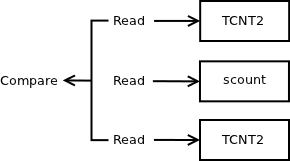
\includegraphics[width=6cm,keepaspectratio]{fig/read.png}
  \caption{Multiple read and result comparison}
  \label{fig:design-read}
\end{figure}

Since setting the current time is possible only within one second precision,
finer time setting must be made using time adjustments.
Section~\ref{sec:sec:analysis-time} explained, that adjusting the time
should use the hardware clock as much as possible.
Adjusting the time changes the value in {\it{OCR2A}} compare register
to delay or shorten the clock tick interval,
which in turn speeds up or slows down the system time.
The default value of the compare register is incremented or decremented by 1
and written to {\it{OCR2A}}.
The number of needed clock ticks to adjust the time for the specified amount
is stored in a variable, that is also updated at each clock tick.
This variable is equal to zero when enough time adjustments were performed,
and the default value of the compare register is written back to {\it{OCR2A}}.
A new call must be developed for the determination of how many such adjustments must be done.

In such a design, a leap second occurrence will be handled just like an unexpected change of time -
the operating system will continue with the wrong system time for some time,
but an NTP client will step or adjust the system time~\cite{ntp-faq}.
This will effectively cause the leap second correction to be applied too late,
which is a trade-off for smaller memory requirements.

%Implemented {\it{clock\_set\_time}} function computes when the system started
%in seconds since the Epoch and saves the result in newly implemented {\it{boottime}} variable.

%Unlike GIT!
%This variable, counting uptime in seconds,
%is particularly used by stimers in Contiki
%and modifying it would lead to misbehaviour of stimer library
%described in section~\ref{sec:contiki-timers}.
